\documentclass{article}
\usepackage[hidelinks]{hyperref}
\usepackage{graphicx}
\usepackage{amsfonts}
\usepackage{amsmath}
\usepackage{enumitem}
\usepackage{polski}
\usepackage[utf8]{inputenc}
\usepackage{indentfirst}
\usepackage{float}
\title{Projekt aplikacji do ekstremalnego uczenia maszynowego do klasyfikacji big data}
\author{Abdelkarim Ahmed, Hernik Aleksandra}
\begin{document}
Wydział Matematyki i Nauk Informacyjnych Politechniki Warszawskiej
\begin{figure}[H]
\begin{center}

\includegraphics[scale=0.5]{MiNI.png}
\end{center}
\end{figure}
\vspace*{\fill}
\begin{center}
\begin{minipage}{.9\textwidth}
\maketitle
\begin{center}Wersja 1.8\end{center}
\end{minipage}
\end{center}
\vfill % equivalent to \vspace{\fill}
\clearpage
\noindent
\begin{table}[H]
\caption{Zmiany w dokumentacji}
\hspace*{-1cm}
\begin{tabular}{|l|l|l|r|}
\hline
\textbf{Data} & \textbf{Autor} & \textbf{Opis zmian} & \textbf{Wersja} \\
\hline
10.10.2016 & Ahmed Abdelkarim & Diagram przypadków użycia & 0.1 \\
10.10.2016 & Aleksandra Hernik & Wstępna wersja harmonogramu i wymagań & 0.2 \\
19.10.2016 & Aleksandra Hernik & Korekty harmonogramu i wymagań & 0.3 \\
02.11.2016 & Ahmed Abdelkarim & Stworzenie i wprowadzenie szablonu & 1.0 \\
02.11.2016 & Ahmed Abdelkarim & Opis przypadków użycia & 1.1 \\
02.11.2016 & Aleksandra Hernik & Opis biznesowy, dokończenie harmonogramu & 1.2 \\
15.11.2016 & Ahmed Abdelkarim & Opis modelu wytwórczego & 1.3 \\
15.11.2016 & Aleksandra Hernik & Architektura rozwiązania & 1.4 \\
15.11.2016 & Ahmed Abdelkarim & Diagram klas & 1.5 \\
12.01.2017 & Ahmed Abdelkarim & Instruckcja i dokumentacja kodu - Python & 1.6 \\
12.01.2017 & Aleksandra Hernik & Instrukcja i dokumentacja kodu - Matlab & 1.7 \\
12.01.2017 & Ahmed Abdelkarim & Przeprowadzone testy, zmiany & 1.8 \\
\hline
\end{tabular}
\end{table}
\tableofcontents
\clearpage
\section{Specyfikacja}
\subsection{Opis biznesowy}
Projekt polega na przygotowaniu dwóch aplikacji. Pierwsza jest napisana w języku Python. Druga została stworzona w środowisku Matlab. Celem obu jest przetestowanie nowego modelu sieci neuronowych - Extreme Learning Machine. Programy zapewniają możliwość wytrenowania sieci neuronowej przy użyciu różnych danych i dostarczają informacje, dotyczące czasu trwania i jakości treningu. Dzięki temu będzie możliwe określenie, czy metoda ELM może być uważana za dobrą alternatywę dla tradycyjnych architektur sieci neuronowych, a także w jakich obszarach sprawdzi się najlepiej. Szczególny nacisk został położony na zbadanie działania dla Big Data.
\subsection{Wymagania funkcjonalne}
\begin{itemize}
\item Przygotowanie danych trenujących i testowych w formie plików csv
\item Trenowanie sieci neuronowej o architekturze ELM
\item Klasyfikacja danych testowych przez wytrenowaną sieć
\item Porównywanie wyników klasyfikacji do spodziewanych rezultatów
\item Analiza jakości klasyfikacji i  czasu trwania treningu
\item Interfejs graficzny
\end{itemize}
Poniższy diagram UML przedstawia zbiór przypadków użycia aplikacji z punktu widzenia użytkownika i systemu. Dotyczy obu aplikacji.
\begin{figure}[H]
\hspace*{-1.5cm}
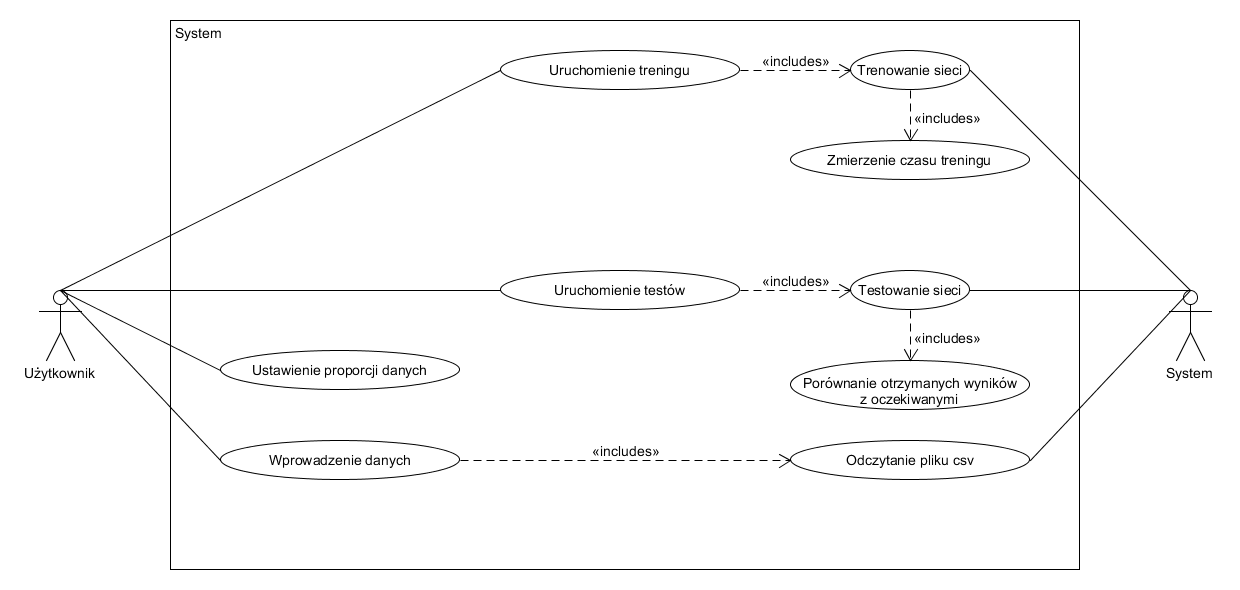
\includegraphics[width=16cm]{use_case.png}
\caption{Diagram przypadków użycia}
\end{figure}
Poniższa tabela zawiera opisy przypadków użycia dla użytkownika oraz odpowiedzi systemu.

\begin{table}[H]
\caption{Opisy przypadków użycia}
\begin{tabular}{|p{3.4cm}|p{5cm}|p{4cm}|}
\hline
\textbf{Nazwa} & \textbf{Opis} & \textbf{Odpowiedź systemu} \\
\hline
Wprowadzenie danych & Wprowadzenie danych używanych do uczenia sieci & Odczytanie pliku csv \\ \hline
Ustawienie proporcji danych & Ustawienie proporcji danych treningowych, testowych i zatwierdzających & Zapisanie wyboru \\ \hline
Uruchomienie treningu & Uruchomienie treningu sieci schematem ELM & Trenowanie sieci i zmierzenie czasu treningu \\ \hline
Uruchomienie testów & Uruchomienie testów sieci wytrenowanej wcześniej schematem ELM & Testowanie sieci i porównanie otrzymanych wyników z oczekiwanymi \\
\hline
\end{tabular}
\end{table}
\clearpage
\subsection{Wymagania niefunkcjonalne}
W poniższej tabeli znajduje się lista wymagań niefunkcjonalnych.
\begin{table}[H]
\caption{Lista wymagań niefunkcjonalnych}
\begin{tabular}{|l|l|p{9.4cm}|}
\hline
\textbf{Obszar} & \textbf{Numer} & \textbf{Opis} \\
\hline
Użyteczność & 1 & Aplikacje muszą działać na komputerach wydziałowych \\
 & 2 & Aplikacje powinny mieć przejrzysty interfejs graficzny \\
 & 3 & Wykresy wyświetlane w aplikacji powinny być czytelne \\
\hline
Wydajność & 4 & Działanie w oparciu o ELM powinno dawać o kilka rzędów wielkości szybszy czas uczenia niż tradycyjne metody \\
\hline 
Inne & 5 & Wykonanie aplikacji w językach Python i MATLAB \\
\hline
\end{tabular}
\end{table}

\subsection{Harmonogram projektu}
\begin{table}[H]
\caption{Harmonogram prac}
\begin{tabular}{|l|r|r|r|}
\hline
\textbf{Etap} & \textbf{Czas} & \textbf{Początek} & \textbf{Koniec} \\
\hline
Przygotowanie pierwszego rozdziału dokumentacji & 24 dni & 10.10.2016 & 02.11.2016 \\
Opracowanie modelu pracy sieci ELM & 14 dni & 17.10.2016 & 30.10.2016 \\
Analiza narzędzi & 7 dni & 31.10.2016 & 06.11.2016 \\
Projekt techniczny & 7 dni & 07.11.2016 & 13.11.2016 \\
Implementacja i napisanie drugiego rozdziału pracy & 14 dni & 07.11.2016 & 20.11.2016 \\
Tworzenie i wykonywanie testów dla small data & 7 dni & 21.11.2016 & 27.11.2016 \\
Tworzenie i wykonywanie testów dla big data & 7 dni & 28.11.2016 & 04.12.2016 \\
Opis wniosków z testów & 7 dni & 05.12.2016 & 11.12.2016 \\
Instrukcja użytkownika & 4 dni & 11.12.2016 & 14.12.2016 \\
\hline
\end{tabular}
\end{table}
\subsection{Architektura rozwiązania}
Zostaną przygotowane dwie niezależne aplikacje pełniące podobne funkcje -- jedna w języku MATLAB, a druga w języku Python. Aplikacje nie posiadają oddzielnych modułów. Aplikacja w MATLABie zostanie przygotowana w formie biblioteki, a aplikacja w Pythonie będzie mieć interfejs graficzny i wykorzystywać zewnętrzną bibliotekę \textit{HP-ELM}. Opracowanie w dalszym ciągu tego rozdziału dotyczy obu aplikacji.

Komponentami aplikacji będą:
\begin{itemize}
\item Sieć - komponent odpowiadający za tworzenie, uczenie i testowanie sieci neuronowej.
\item Preprocesor - komponent przygotowujący dane treningowe i testowe dla sieci. Jego funkcjami są wczytanie plików, konwersja na wygodny format, podział na dane treningowe i testowe oraz normalizacja danych.
\item Benchmark - komponent zajmujący się korzystaniem z sieci na konkretnych danych i zbieraniem informacji na temat wyników.
\end{itemize}
Poniżej prezentowana jest struktura klas aplikacji.

\begin{figure}[H]
\hspace*{-2cm}
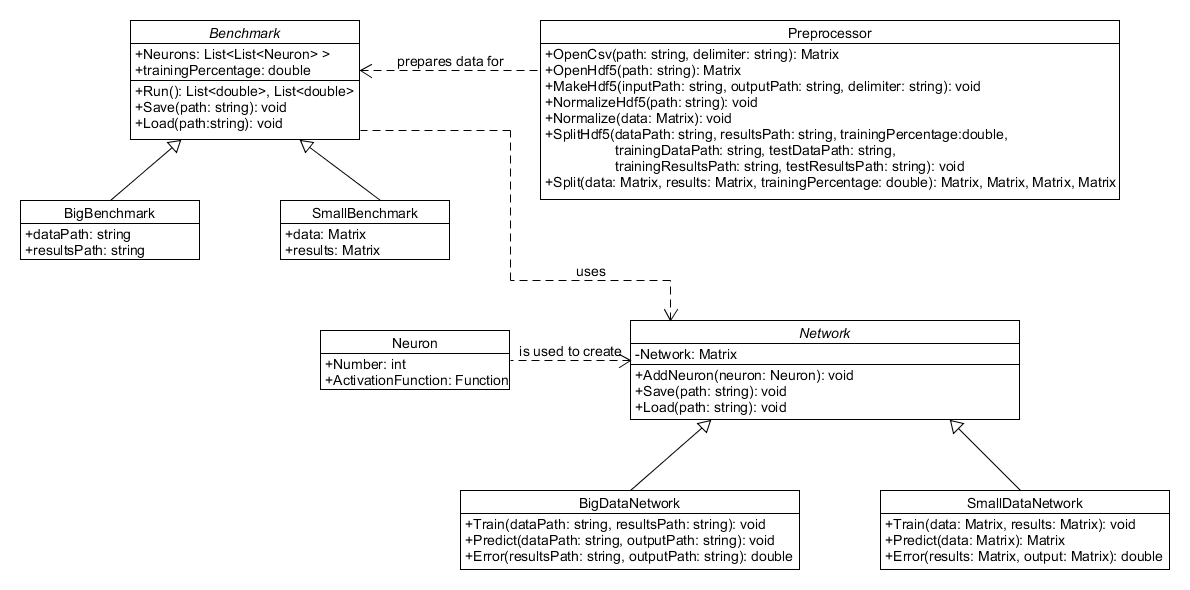
\includegraphics[width=16cm]{classes.png}
\caption{Diagram klas}
\end{figure}

Uszczegółowienie opisu dla wybranych funkcji:
\begin{itemize}
\item Benchmark.Run zwraca listę czasów treningów i błędów dla przypadku testowego.
\item Preprocessor.Split dzieli dane na treningowe i testowe. Analogiczna do SplitHdf5, ale dla małych danych.
\item Big/SmallDataNetwork.Error zwraca błąd klasyfikacji na podstawie oczekiwanych i rzeczywistych rezultatów.
\end{itemize}

\subsection{Model wytwórczy}
Wybranym modelem wytwórczym jest model ewolucyjny, ponieważ stworzenie programu nie jest celem tej pracy inżynierskiej, a jedynie środkiem pozwalającym go osiągnąć. Ponadto do aplikacji prawdopodobnie będą dodawane funkcjonalności wraz z pojawianiem się nowych pomysłów związanych z powstawaniem dalszych części pracy. Zaistniała sytuacja spowoduje, że z punktu widzenia biznesowego osoby tworzące aplikacje są również klientami, a stawianie wymagań jest jednocześnie analizą i projektowaniem -- oddzielenie tych faz byłoby sztuczne i jedynie spowalniałoby pracę. Oprócz tego, stawianie nowych wymagań (połączone z analizą i projektowaniem) może odbywać się równolegle z implementacją. Wersją końcową projektu jest ostatnia wersja, która zostanie wykorzystana w trakcie tworzenia pracy inżynierskiej.

\subsection{Uwagi}
\begin{itemize}
\item Automatyczne testy, sprawdzające główną funkcjonalność programu - trening sieci - nie zostaną utworzone. Istotą projektu jest przeanalizowanie otrzymywanych, a nie otrzymanie z góry zaplanowanych wyników.
\item Nie zostały postawione wymagania związane z niezawodnością i utrzymaniem. Aplikacje służą wyłącznie jako narzędzia do przetestowania nowej technologii, więc jedynym wymaganiem jest działanie w momencie przeprowadzania testów. Ta kwestia może ulec zmianie, jeśli testy wypadną korzystnie dla ELM.
\item Wydajność jest raczej oczekiwaniem, nie wymaganiem. Z prac, na których bazowany jest projekt wynika, że metoda powinna być szybka, jednak założenia projektu polegają na sprawdzeniu, a nie przyjęciu tej tezy. Ponadto nie zostały zaimplementowane inne metody uczenia sieci neuronowych, więc precyzyjna ocena wydajności byłaby trudna.
\item Ponieważ aplikacje nie są ze sobą połączone, a same również nie składają się z modułów, problem integracji zostaje pominięty.
\end{itemize}
\clearpage
\section{Instrukcja użytkownika}
\subsection{Aplikacja sieci ELM w Pythonie}
\subsubsection*{Przygotowanie}
Aplikacja sieci ELM w Pythonie wymaga zainstalowania najnowszej wersji Pythona 2 wraz ze standardowymi bibliotekami -- najprostszym sposobem jest zainstalowanie pakietu Anaconda. Oprócz tego, należy zainstalować bibliotekę \textit{HP-ELM} -- należy uruchomić konsolę z uprawnieniami administratora i wywołać polecenie \textit{pip install hpelm}. 
\subsubsection*{Uruchomienie aplikacji}
Aby uruchomić aplikację, należy za pomocą folderu przejsć do katalogu zawierającego pliki aplikacji i wywołać polecenie \textit{python test.py}. W przypadku niektórych systemów operacyjnych (na przykład Arch Linux) może być konieczne użycie zamiast tego polecenia \textit{python2 test.py}.
\subsubsection*{Użytkowanie aplikacji}
Bezpośrednio po uruchomieniu powinien pojawić się ekran jak na rysunku \ref{python_ekran}.
\begin{figure}[H]
\centering
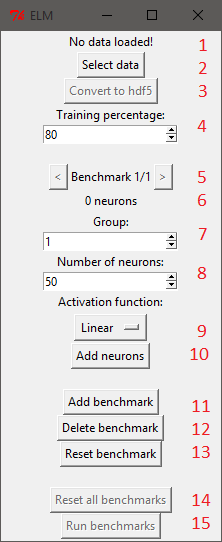
\includegraphics{instrukcja_python_start.png}
\caption{Ekran aplikacji}
\label{python_ekran}
\end{figure}
Zawiera elementy oznaczone tu liczbami od 1 do 15:
\begin{enumerate}
\item nazwa załadowanego pliku z danymi,
\item wybór danych -- uruchamia dwa okienka umożliwiające wybór pliku z danymi w formacie \textit{csv} (dla small data) i \textit{hdf5} (dla big data) -- pierwsze okienko to wybór danych wejściowych, a drugie okienko to wybór oczekiwanych wyników,
\item konwersja wczytanych danych do \textit{hdf5} -- pozwala na utworzenie plików \textit{hdf5} zgodnych z aplikacją, na przykład w celu zasymulowania obliczeń big data,
\item procent danych treningowych,
\item obecnie wybrany benchmark oraz kontrolki pozwalające przełączać się między benchmarkami,
\item liczba neuronów w obecnym benchmarku,
\item grupa, do której należy obecny benchmark,
\item liczba neuronów do dodania do obecnego benchmarku,
\item funkcja aktywacji dla neuronów do dodania do obecnego benchmarku,
\item dodanie określonych powyżej neuronów,
\item dodanie nowego benchmarku (przypisanego do tej samej grupy, co obecny benchmark),
\item usunięcie obecnego benchmarku,
\item usunięcie wszystkich neuronów z obecnego benchmarku,
\item usunięcie wszystkich benchmarków,
\item uruchomienie benchmarków.
\end{enumerate}
Aby skorzystać poprawnie z aplikacji, należy najpierw wybrać dane, ustalić procent danych treningowych, dodać tyle benchmarków, ile się chce (w każdym musi być co najmniej jeden neuron), przypisać im odpowiednie grupy, aby podzielić otrzymane wyniki na różne serie danych, a następnie wcisnąć przycisk \textit{Run benchmarks}. Efektem jest pojawienie się nowego okienka z wykresami opisującymi wyniki eksperymentu, jak na rysunku \ref{instrukcja_python_end}.
\begin{figure}[H]
\centering
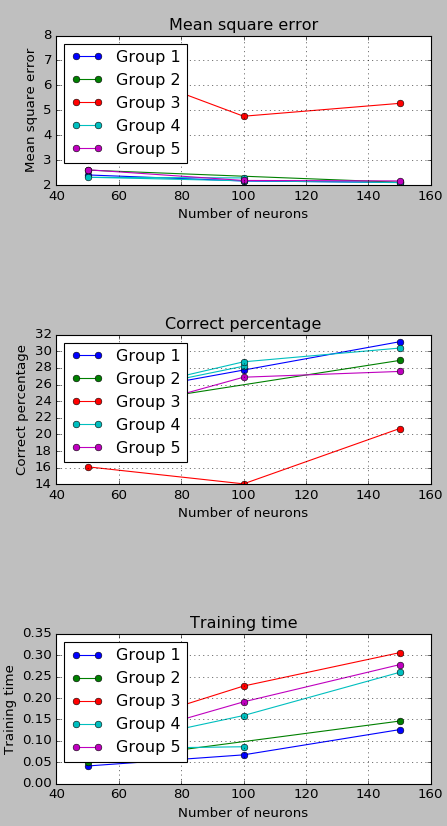
\includegraphics[width=0.8\textwidth]{instrukcja_python_end.png}
\caption{Przykładowe wyniki działania aplikacji}
\label{instrukcja_python_end}
\end{figure}
\clearpage
\subsection{Aplikacja sieci ELM w Matlabie}
\subsubsection*{Przygotowanie}
Aby uruchomić aplikację, należy skorzystać z programu Matlab.
Aplikacja składa się z dwóch plików: klasy sieci, zawierającej implementację algorytmu (\textit{ELM.m}) i przykładowego skryptu wywołującego kolejne funkcje tej klasy (\textit{ELM\textunderscore run.m}).
Konieczne jest ustawienie folderu roboczego na folder, w którym znajdują się te pliki.
\subsubsection*{Użytkowanie aplikacji}
Uruchomienie aplikacji polega na wywołaniu skryptu \textit{ELM\textunderscore run.m}, jednak najpierw należy ustawić wszystkie konieczne parametry. Rysunek \ref{elm_run} przedstawia kod skryptu \textit{ELM\textunderscore run.m} z pominięciem części odpowiedzialnej za komunikację z użytkownikiem.
\begin{figure}[H]
\centering
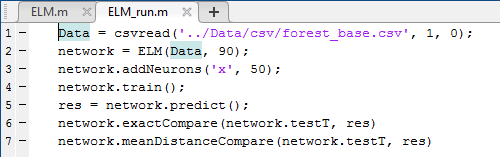
\includegraphics[width=1\textwidth]{elm_run.png}
\label{elm_run}
\caption{Skrypt \textit{ELM\textunderscore run.m}}
\end{figure}
Znaczenie i możliwe modyfikacje kolejnych linii:
\begin{enumerate}
\item Przygotowanie danych wejściowych.
W tym wypadku dane są wczytywane z pliku csv, co nie jest konieczne.
Wymagane jest jedynie, żeby dane wejściowe następnej funkcji były macierzą, w której $n$ kolumn oznacza cechy, a jedna (ostatnia) klasy, do których należą próbki. Wartości wszystkich cech i klas muszą być liczbami.
\item Konstruktor klasy sieci. 
Pierwszy argument to wspomniana wcześniej tablica. 
Drugi oznacza procent danych przeznaczonych do treningu sieci.
Pozostałe dane (w tym wypadku 10\%) to dane testowe.
\item Dodawanie neuronów.
Pierwszy argument to funkcja aktywacji.
Może to być dowolny kod wykonywalny w Matlabie, gdzie zmienną jest x.
Drugi argument to liczba neuronów tego typu.
Ta funkcja może zostać wywołana dowolnie wiele razy, aby stworzyć neurony o różnych funkcjach aktywacji.
\item Rozpoczęcie treningu sieci. 
Funkcja wykorzystuje dane wybrane w drugim kroku jako treningowe.
Należy ją wywołać po dodaniu wszystkich neuronów.
\item Klasyfikacja danych testowych.
Wynikiem jest wektor klas - po jednej dla każdego obiektu, należącego do danych testowych.
\item Funkcja porównująca wynik uzyskany w poprzednim kroku z oczekiwaniami.
Przyjmuje jako argumenty wektor z danymi oczekiwanymi (zapisany wcześniej przez aplikację jako pole klasy) i wektor wynikowy klasyfikacji.
Funkcja zwraca liczbę z zakresu $[0, 1]$, oznaczającą jaka część próbek została sklasyfikowana poprawnie.
\item Inna funkcja poprawności klasyfikacji, przyjmująca takie same argumenty.
Zwraca średnią odległość klas przewidzianych od faktycznych.
Ta miara może być użyteczna, jeśli klasy o bliskich numerach są bardziej zbliżone niż o dalekich.
\end{enumerate}
Po odpowiednim zmodyfikowaniu skryptu i uruchomieniu go otrzymujemy wynik (rys. \ref{elm_run_result}) - informacje o czasie trwania i skuteczności treningu.
\begin{figure}[H]
\centering
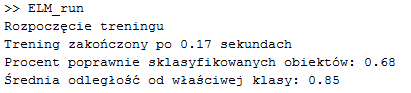
\includegraphics[width=0.9\textwidth]{elm_results.PNG}
\caption{Wynik wywołania skryptu}
\label{elm_run_result}
\end{figure}
\clearpage
\section{Dokumentacja kodu}
\subsection{Aplikacja sieci ELM w Pythonie}
Aplikacja sieci ELM w Pythonie składa się z plików:
\begin{itemize}
\item \textit{benchmark.py},
\item \textit{error.py}, 
\item \textit{preprocessor.py},
\item \textit{test.py}.
\end{itemize}
Ponadto wykorzystywane są biblioteki:
\begin{itemize}
\item \textit{HP-ELM}
\item \textit{numpy}
\item \textit{sklearn}
\item \textit{h5py}
\item \textit{matplotlib}
\end{itemize}
Plik \textit{test.py} to główny plik aplikacji, w którym zdefiniowane jest rozmieszczenie interfejsu użytkownika oraz funkcje wywoływane przy naciśnięciu odpowiednich jego elementów, takie jak zapamiętywanie dodanych neuronów, uruchomienie testu i rysowanie wykresów.

W pliku \textit{preprocessor.py} znajduje się zestaw funkcji odpowiedzialnych za wstępne przetwarzanie danych:
\begin{itemize}
\item \textbf{open\textunderscore csv}(\textit{path}) -- otwiera plik \textit{csv} (rozdzielony przecinkami) ze ścieżki \textit{path} i zwraca utworzoną na jego podstawie macierz
\item \textbf{normalize}(\textit{data}) -- zwraca znormalizowane dane z macierzy \textit{data}
\item \textbf{normalize\textunderscore hdf5}(\textit{data\textunderscore path}, \textit{output\textunderscore path}) -- normalizuje dane z pliku \textit{data\textunderscore path} w formacie \textit{hdf5} do pliku \textit{output\textunderscore path}.
\item \textbf{split}(\textit{data}, \textit{results}, \textit{training\textunderscore percentage}) -- dzieli dane wskazane w macierzy \textit{data} i \textit{results} na dane i rezultaty treningowe oraz testowe w zależności od \textit{training\textunderscore percentage}, zwraca dane treningowe, dane testowe, rezultaty treningowe i rezultaty testowe.
\item \textbf{split\textunderscore hdf5}(\textit{data\textunderscore path}, \textit{results\textunderscore path}, \textit{training\textunderscore percentage}, \textit{training\textunderscore data\textunderscore path}, \textit{test\textunderscore data\textunderscore path}, \textit{training\textunderscore results\textunderscore path}, \textit{test\textunderscore results\textunderscore path}) -- analogicznie do funkcji \textbf{split} dzieli dane znajdujące się w plikach \textit{hdf5} do odpowiednich plików wynikowych.
\end{itemize}
Plik \textit{error.py} rozszerza funkcjonalność biblioteki \textit{HP-ELM} o dodatkowy sposób liczenia błędu klasyfikacji za pomocą funkcji:
\begin{itemize}
\item \textbf{percentage}(\textit{expected}, \textit{actual}) -- zwraca procent poprawnie sklasyfikowanych próbek na podstawie macierzy \textit{expected} (oczekiwane wyniki) i \textit{actual} (rzeczywiste wyniki).
\item \textbf{hdf5\textunderscore percentage}(\textit{expected\textunderscore path}, \textit{actual\textunderscore path} -- analogicznie do funkcji \textbf{percentage}, dla wskazanych plików \textit{hdf5}.
\end{itemize}

W pliku \textit{benchmark.py} zdefiniowana została klasa \textbf{Benchmark}, która automatyzuje uruchamianie testów i ma następujące metody:
\begin{itemize}
\item \textbf{\textunderscore \textunderscore init\textunderscore \textunderscore}(\textit{self}, \textit{name}, \textit{training\textunderscore percentage}, \textit{neurons}) -- konstruktor, tworzący instancję klasy \textbf{Benchmark} z uzupełnionymi odpowiednimi polami. Nie powinien być wywoływany bezpośrednio.
\item \textbf{small\textunderscore benchmark}(\textit{name}, \textit{training\textunderscore percentage}, \textit{neurons}, \textit{data}, \textit{results}) -- statyczna metoda tworząca obiekt klasy \textbf{Benchmark} przystosowany do obliczeń small data (na macierzach w pamięci, wczytanych z plików \textit{csv}). Ustawia nazwę, procent danych treningowych, zestaw benchmarków (listę zawierająca zestawy neuronów dla każdego z nich), dane i oczekiwane wyniki.
\item \textbf{big\textunderscore benchmark}(\textit{name}, \textit{training\textunderscore percentage}, \textit{neurons}, \textit{data\textunderscore path}, \textit{results\textunderscore path}, \textit{output\textunderscore path}) -- statyczna metoda działająca analogicznie do \textbf{small\textunderscore benchmark}, ale dla obliczeń big data (na plikach \textit{hdf5}). 
\item \textbf{run}(\textit{self}) -- uruchamia benchmark i zwraca błędy średniokwadratowe, procent poprawnie sklasyfikowanych danych i czas trwania treningu.
\end{itemize}
\subsection{Aplikacja sieci ELM w Matlabie}
Aplikacja sieci ELM w Matlabie składa się z dwóch plików: \textit{ELM.m}, zawierającego implementację sieci neuronowej, oraz skryptu \textit{ELM\textunderscore run.m}, służącego jako przykładowe wywołanie -- opisany dokładnie został w instrukcji użytkownika.

W pliku \textit{ELM.m} zaimplementowała została klasa \textbf{ELM}, która zapewnia wszystkie funkcjonalności biblioteki. Zawiera metody:
\begin{itemize}
\item \textbf{ELM}(\textit{data}, \textit{trainingPercentage}) -- tworzy obiekt klasy ELM z danymi \textit{data} -- macierzą, która w ostatniej kolumnie zawiera oczekiwane wyniki, dzieląc je na dane treningowe i testowe według \textit{trainingPercentage}.
\item \textbf{addNeurons}(\textit{obj}, \textit{funcStr}, \textit{num}) -- dodaje do sieci \textit{num} neuronów z funkcją aktywacji opisaną w \textit{funcStr} (napis opisujący dowolną funkcja od zmiennej x, na przykład 'x * x').  
\item \textbf{normalize}(\textit{~}, \textit{data}) -- zwraca znormalizowane dane z macierzy \textit{data}.
\item \textbf{train}(\textit{obj}) -- trenuje sieć.
\item \textbf{predict}(\textit{obj}) -- uruchamia test (wymaga uprzedniego wytrenowania sieci).
\item \textbf{exactCompare}(\textit{~}, \textit{actualT}, \textit{predictedT}) -- zwraca część (liczbę od 0 do 1) poprawnie sklasyfikowanych próbek, gdzie \textit{actualT} i \textit{predictedT} to odpowiednio rzeczywiste i otrzymane wyniki.
\item \textbf{meanDistanceCompare}(\textit{~}, \textit{actualT}, \textit{predictedT}) -- zwraca średni moduł z różnicy między rzeczywistymi i otrzymanymi wynikami.
\item \textbf{parseData}(\textit{~}, \textit{d}) -- przetwarza macierz \textit{d}, zwracając \textit{X} -- dane wejściowe i \textit{T} -- oczekiwane wyniki, znajdujące się w ostatniej kolumnie \textit{d}.
\item \textbf{createH}(\textit{obj}, \textit{X}) -- wyznacza macierz \textit{H}, używaną w wewnętrznych obliczeniach ELM -- dokładny opis celu i sposobu obliczania \textit{H} znajduje się w pracy inżynierskiej.
\end{itemize}
\clearpage
\section{Przeprowadzone testy}
Obie aplikacje były testowane na dwóch zestawach danych: zestawie 50000 próbek składających się z 10 cech i zestawie 15120 próbek składających się z 54 cech. Przeprowadzane testy obejmowały uruchamianie sieci przy różnych liczbach neuronów (z zakresu od 1 do 2400, a także próba dla 10000 neuronów) i funkcjach aktywacji -- w tym mieszanych (na przykład 10 neuronów liniowych i 5 neuronów sigmoidalnych). Dla żadnej kombinacji neuronów w żadnej z aplikacji nie wystąpił błąd, a obliczenia nie zajmowały więcej niż kilkanaście sekund, z wyjątkiem testu 10000 neuronów, który nie zakończył się po 10 minutach -- jest to jednak zgodne z oczekiwaniami wobec ELM. Dokładne wyniki dostępne są w pracy inżynierskiej.
\clearpage
\section{Zmiany w stosunku do pierwotnych założeń}
Główną zmianą w stosunku do początkowych założeń było stworzenie aplikacji w MATLABie jako biblioteki z własną implementacją ELM, a nie identycznej aplikacji jak w Pythonie -- związku z tym nie było potrzeby tworzenia klasy \textbf{Benchmark} w tej implementacji.

Wszystkie zaplanowane funkcjonalności zostały zaimplementowane, a ponadto aplikacja w Pythonie została rozszerzona o:
\begin{itemize}
\item wczytywanie plików \textit{hdf5},
\item konwersja danych z \textit{csv} do \textit{hdf5}
\item planowanie wielu testów naraz.
\end{itemize}
Spełnione zostały również wszystkie wymagania niefunkcjonalne, z wyjątkiem przejrzystego interfejsu graficznego w przypadku aplikacji w MATLABie (ze względu na zmianę jej charakteru).

Uległ zmianie harmonogram -- implementacja i napisanie drugiego rozdziału pracy przedłużyła się do 14.12.2016, instrukcja użytkownika została napisana przed stworzeniem i wykonaniem testów, które z kolei zajęły tylko tydzień. Dalszy czas został poświęcony na dopracowanie pracy.
\clearpage
\section{Wykaz ważniejszych oznaczeń i akronimów}
\begin{itemize}[label={},leftmargin=*]
\item Big Data -- dane z liczbą próbek tak dużą, że nie występuje efekt przeuczenia
\item ELM -- \textbf{E}xtreme \textbf{L}earning \textbf{M}achine - ekstremalne uczenie maszynowe
\item Small Data -- dane, dla których jest za mało próbek, aby sieć poznała dokładnie model bez przeuczenia
\item Toolbox -- zbiór funkcji stworzonych we wspólnym celu; biblioteka;
\end{itemize}

\end{document}